\documentclass[journal,twoside,web]{template/ieeecolor2-tectonic}
\usepackage{template/generic}
\def\logoname{template/LOGO-generic-web}
\usepackage{cite}
\usepackage{amsmath,amssymb,amsfonts}
\usepackage{graphicx}
\usepackage{booktabs}
\usepackage{array}
\usepackage{url}

\def\journalname{IEEE Transactions on Biomedical Engineering}
\markboth{\journalname, VOL.~XX, NO.~XX, 2026}
{[TODO: Author] \MakeLowercase{\textit{et al.}}: An End-to-End Motor-Imagery Brain--Computer Interface}

\begin{document}

\title{An End-to-End Motor-Imagery Brain--Computer Interface: From Low-Cost Acquisition and Deployed Classical Decoding to a Reproducible Benchmark of Compact Coordinate-Field Networks}

\author{[TODO: Insert verified author names and order]
\thanks{[TODO: Insert affiliations, correspondence address, and author e-mail addresses.]}
\thanks{[TODO: Insert all financial support and grant identifiers, or an explicit statement that no external funding supported the work.]}}

\maketitle

\begin{abstract}
\textit{Objective:} To present a complete motor-imagery (MI) electroencephalography (EEG) platform---low-cost acquisition, a deployable online decoding pipeline, and compact neural architectures---and to evaluate its classical and neural decoders under auditable protocols.
\textit{Methods:} The platform pairs a 16-channel consumer-grade amplifier with custom cue-presentation software and an online pipeline that couples aligned classical decoders (Euclidean-aligned filter-bank common spatial patterns; Riemannian tangent space) with unsupervised calibration, decision-boundary recentering, and temporal evidence gating for closed-loop assistive control. Offline, 43 neural configurations were evaluated on five cohorts (132 participant--dataset units; 26,574 trials) under one frozen recipe with five seeds, source-only scaling, validation-selected training, seeded refitting, one test pass, and exact job-level audit.
\textit{Results:} On the locally acquired cohort, the deployed classical pipeline reached 91.1$\pm$6.3\% within-participant and 86.4$\pm$8.2\% leave-one-participant-out accuracy. All 96,320 benchmark jobs passed audit. The highest observed balanced accuracy was 73.99\% for a 32,042-parameter coordinate-field continuation, versus 73.32\% for the 75,668-parameter TCFormer reference (exploratory difference 0.67 points; 95\% bootstrap interval $-0.43$ to 1.90; adjusted $P=0.772$); a 13,523-parameter compact alternative reached 73.67\%. The reference was better calibrated.
\textit{Conclusion:} The platform supports accurate deployed classical decoding, and compact coordinate-field networks are efficiency-competitive with a recent large transformer reference at less than half its parameters, without a confirmatory superiority claim.
\textit{Significance:} The work provides an auditable path from electrode to command, with compact decoders suited to embedded closed-loop use.
\end{abstract}

\begin{IEEEkeywords}
Brain--computer interface, compact neural network, electroencephalography,
motor imagery, reproducibility, spatial coordinates.
\end{IEEEkeywords}

\section{Introduction}
\label{sec:introduction}

Motor-imagery electroencephalography (EEG) decoding is complicated by low signal-to-noise ratio, limited trials per participant, and substantial variation across participants, sessions, acquisition systems, and electrode layouts. Most published work isolates one link of the chain---usually the classifier---although practical brain--computer interface (BCI) performance is set by the whole system: the acquisition hardware and cue protocol that produce the training data, the alignment and calibration steps that bridge sessions, the temporal evidence gating that turns noisy per-window probabilities into safe discrete commands, and the decoder itself. This paper presents and evaluates that complete chain.

Classical methods combine spatial or covariance representations with comparatively simple classifiers. Filter-bank common spatial patterns (FBCSP) remain a widely used spectral--spatial reference \cite{Ang2012}, covariance geometry supports tangent-space classifiers \cite{Barachant2012}, and Euclidean alignment (EA) is an established train-only adaptation strategy for reducing domain mismatch \cite{He2020}. These methods are computationally light, data-efficient, and---as we show---remain strong when embedded in a deployed online pipeline.

Deep models instead learn temporal, spatial, or attention-based representations directly from trials. Representative families include compact depthwise networks \cite{Lawhern2018}, convolutional networks \cite{Schirrmeister2017}, filter-bank multi-view models \cite{Mane2021,Liu2023}, temporal convolutional models \cite{Ingolfsson2020}, and convolution--attention hybrids \cite{Song2023,Altaheri2023,Zhao2024,Altaheri2025}. Their published numbers are difficult to compare directly because dataset subsets, preprocessing, split construction, validation use, seed counts, and aggregation frequently differ. Reproducible comparison therefore requires the prediction boundary, data provenance, aggregation estimator, and model-selection status to be fixed and audited \cite{Jayaram2018,Pineau2021}.

Most spatial neural operators are indexed by channel order: they work on a fixed montage but do not define how a learned spatial weight should be evaluated at an electrode coordinate absent during training. We investigate a narrower alternative: parameterize spatial weights as a regularized radial-basis field over spherical electrode coordinates, sample that field at the observed positions, and attach a compact energy-and-dynamics continuation to a filter-bank convolutional floor. The field parameterizes weights, not EEG trials or labels.

This work makes four contributions. First, it documents an end-to-end MI-BCI platform: a 16-channel consumer-grade acquisition rig with custom cue software, and an online pipeline with unsupervised calibration, decision-boundary recentering, and temporal evidence gating, used for closed-loop assistive navigation. Second, it reports the deployed classical decoders---EA-FBCSP and Riemannian tangent space---under within-participant and leave-one-participant-out protocols on the locally acquired cohort. Third, it reports a common-recipe benchmark of 43 neural configurations across five motor-imagery cohorts with five fixed seeds and exact job-level accounting, in which two in-house compact coordinate-field models are efficiency-competitive with the prespecified public comparator (TCFormer) at a fraction of its parameters. Fourth, it reports participant-aware uncertainty, calibration, parameter count, inference latency, memory, and runtime rather than treating accuracy as the only outcome. Because the benchmark contains no independent confirmation cohort and the observed leader was selected among 43 configurations, all leader comparisons are exploratory; scope limits are consolidated in Section~\ref{sec:discussion}.

\section{Methods}
\label{sec:methods}

\subsection{Acquisition Platform and Cue Paradigm}
\label{sec:platform}

Local recordings were acquired with an OpenBCI Cyton+Daisy biosensing amplifier (16 channels, 125~Hz, 24-bit) streaming over a serial radio link. Fifteen passive electrodes were placed at sites of the international 10--20 system emphasizing sensorimotor and surrounding cortex (Cz, Pz, C3, C4, P7, P8, Fz, F7, F8, F3, F4, T7, T8, P3, P4), with one amplifier input unused. A custom full-screen cue application controls each recording: after a 10-s preparation period, each trial presents a 2-s planning cue, a 2-s imagery (task) window, and a 2-s rest interval. Each run contains 60 trials balanced 30/30 between left- and right-hand imagery in shuffled order; each participant contributed four runs in one seated session. Hardware event markers are injected into the amplifier stream at every phase transition, and runs are stored as annotated MNE-Python raw files \cite{Gramfort2013} together with the exact cue-timing configuration. Figure~\ref{fig:platform} summarizes the platform.

\begin{figure*}[t]
\centering
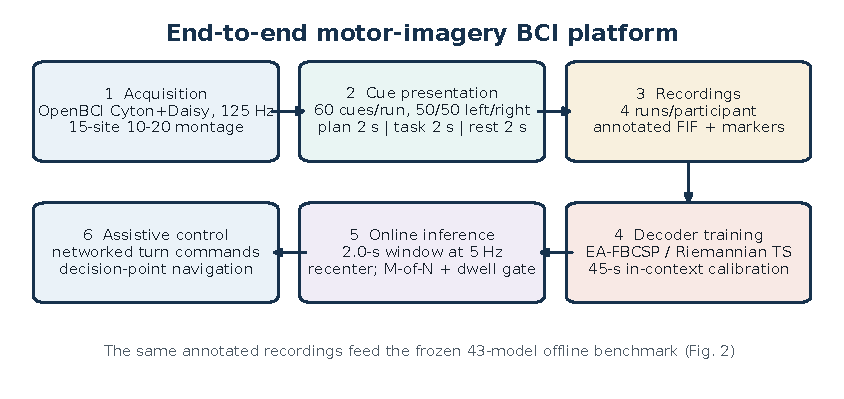
\includegraphics[width=0.98\textwidth]{figures/platform.pdf}
\caption{End-to-end motor-imagery BCI platform. A low-cost 16-channel acquisition rig and cue-presentation application produce annotated training recordings; the online pipeline trains aligned classical decoders, calibrates without labels in the use context, and gates per-window evidence into discrete assistive commands. The same recordings feed the offline benchmark of Fig.~\ref{fig:workflow}.}
\label{fig:platform}
\end{figure*}

\subsection{Online Decoding Pipeline and Closed-Loop Use}
\label{sec:online}

The online decoder consumes 2.0-s windows at a 0.2-s stride (five decisions per second). Each window is filtered by a causal minimum-phase FIR filter bank with four bands (8--12, 11--15, 14--20, and 20--30~Hz). Two interchangeable decoders share one interface. The EA-FBCSP decoder whitens each band by the inverse square root of that band's mean trial covariance, computed per recording during training \cite{He2020}, extracts two CSP log-variance components per band \cite{Ang2012}, and classifies with shrinkage linear discriminant analysis \cite{LedoitWolf2004}. The Riemannian decoder estimates Ledoit--Wolf-regularized covariance per band, recenters each training recording to the identity by congruence with the inverse square root of its geometric mean, projects to the affine-invariant tangent space, and classifies with logistic regression \cite{Barachant2012}.

Deployment begins with a 45-s unsupervised calibration in the use context: the alignment reference (EA whitener or Riemannian mean) is recomputed from unlabeled live data, absorbing the training-to-use distribution shift without touching decoder weights, and the decision-boundary neutral point is seeded from the median calibration log-odds. During use, decisions are taken on the recentered margin; a configuration toggle either freezes the boundary at its calibration seed or tracks slow drift with a rest-gated, clamped exponential update. Per-window predictions pass a confidence floor (0.85), an M-of-N vote (4 of 5 windows), and a dwell requirement (three consecutive consensus windows) before a discrete command is emitted over a local network socket.

The pipeline drives a simulated differential-drive assistive robot through randomized corridor courses, each comprising 40 decision junctions: the robot advances autonomously, halts at each junction, and waits for a gated left/right command; wrong turns are recoverable. In pilot closed-loop sessions (four participants, 16 randomized courses), every course was completed, with 92.0\% of junctions passed on the first command and a median command latency of 0.2~s; a companion manuscript reports that study in full. \textbf{[TODO: cite or reference the companion closed-loop study according to its publication status, and disclose the overlap to the editor.]}

\subsection{Benchmark Cohorts and Evaluation Boundaries}

The offline benchmark used five already-opened development cohorts (Table~\ref{tab:datasets}). The two BCI Competition IV datasets were obtained from the authoritative BNCI record and retain their official session or chronological boundaries \cite{Tangermann2012,Leeb2007}. Cho2017 was obtained through its supporting-data record \cite{Cho2017,ChoData2017}. The PhysioNet EEG Motor Movement/Imagery Database was used at version 1.0.0, with acquisition context provided by BCI2000 \cite{Schalk2009,Schalk2004}. For each public source, the reproducible data contract records source URL and version, access date, exact file names and hashes, captured terms, ordered channels, event mapping, preprocessing identity, and cache hashes. Raw and transformed EEG remain outside the code repository.

Local Exp4 is the platform cohort of Section~\ref{sec:platform}: eight pseudonymous participants with four chronological recordings each (participant S10 used the analogous recordings 5--8 after an invalidated first session). Recordings 1--2 were training, recording 3 was validation, and recording 4 was the prediction-only test recording. The registered task was binary left- versus right-hand imagery. \textbf{[TODO---RELEASE BLOCKER: insert the institution, protocol title and number, approval or exemption status, effective dates, consent basis, recruitment population, demographics, data controller, and written authorization for publication of aggregate results.]}

\begin{table*}[t]
\caption{Frozen Common-Grid Dataset Protocol}
\label{tab:datasets}
\centering
\scriptsize
\setlength{\tabcolsep}{3.4pt}
\begin{tabular}{p{2.35cm}rrrp{1.8cm}p{2.0cm}p{1.5cm}p{5.0cm}}
\toprule
Dataset & Participants & Trials & Classes & EEG inputs & Analysis epoch & Samples & Frozen partition \\
\midrule
Local Exp4 & 8 & 1,920 & 2 & 15 monopolar channels & 0.0--2.0 s & 256 & Chronological recordings: two train, one validation, one prediction-only test \\
BNCI2014-001 & 9 & 5,184 & 4 & 21 selected of 22 & 0.5--3.0 s & 320 & Per participant: 240 train, 48 validation, 288 official-session test trials \\
BNCI2014-004 & 9 & 6,520 & 2 & 3 supplied bipolar derivations & 0.5--3.0 s & 320 & Official chronology; 240--280 train, 160 validation, and 280--320 test trials per participant \\
Cho2017 & 52 & 10,520 & 2 & 21 selected & 0.5--3.0 s & 320 & Five rotating acquisition-order block folds; 120/144 train, 40/48 validation, 40/48 test trials per fold \\
PhysioNet S1--S54 & 54 & 2,430 & 2 & 21 selected of 64 & 0.5--3.0 s & 320 & Imagery runs 4, 8, and 12 rotate through train, validation, and test; 15 trials per role \\
\bottomrule
\end{tabular}
\end{table*}

The five datasets contribute 132 participant--dataset units and 26,574 unique trials. Cho2017 contributes five folds per participant and PhysioNet three; the other datasets contribute one held-out split, producing 448 participant/fold units. A fold is a repeated measurement within participant, not an independent sample.

\subsection{Preprocessing and Leakage Control}

The common public profile applied a 4--40-Hz passband, extracted the half-open interval 0.5--3.0~s relative to the declared event interval, resampled to 128~Hz, demeaned each epoch, and produced 320 samples. A symmetric common-average reference was applied over the selected 21 channels except for BNCI2014-004, whose three inputs are supplied bipolar derivations. Local Exp4 used its shorter task-valid profile: 4--40~Hz, the half-open interval 0.0--2.0~s, resampling from 125 to 128~Hz, 256 samples, epoch demeaning, and common-average reference over 15 channels.

Channel scaling was strictly source-only. During model selection, each scaler was fitted to training rows and applied unchanged to validation and test rows. For the final refit, a new scaler was fitted to the union of training and validation data; held-out test rows never determined scaling. Test labels were excluded from preprocessing choices, stopping, epoch selection, refit, and calibration. Figure~\ref{fig:workflow} summarizes the frozen flow from acquisition records to audited aggregate estimates; immutable identities link each job to the dataset cache, split, model configuration, seed, environment, and prediction artifact.

\begin{figure*}[t]
\centering
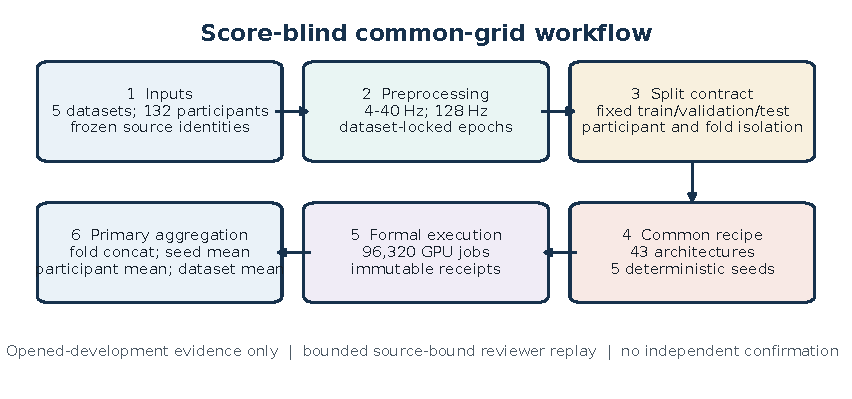
\includegraphics[width=0.98\textwidth]{figures/workflow.pdf}
\caption{Frozen benchmark workflow. Public data are acquired from authoritative records into a private, identity-hashed cache; Local Exp4 remains under its institutional authorization. Source-only scaling, validation selection, seeded reset, train-plus-validation refit, and one-shot test prediction precede exact audit and participant-aware aggregation.}
\label{fig:workflow}
\end{figure*}

\subsection{Common Neural Model Grid}

The common grid contained 43 neural architecture/configuration rows: 15 public reference configurations and 28 in-house coordinate-field configurations (including their channel-indexed controls). Public families included EEGNet, shallow and deep convolutional networks, EEG-Conformer, ATCNet, FBCNet, EEG-TCNet, FBMSNet, CTNet, EEGSym, and TCFormer \cite{Lawhern2018,Schirrmeister2017,Song2023,Altaheri2023,Mane2021,Ingolfsson2020,Liu2023,Zhao2024,PerezVelasco2022,Altaheri2025}. Public architectures were adapted only at the input/output interface and trained under the same benchmark recipe; a common-recipe result is not an author-recipe reproduction. TCFormer was the prespecified public comparator; its runtime snapshot was hash-pinned to the upstream source.

\subsubsection{Coordinate-field spatial operator}

Let $q_1,\ldots,q_A\in\mathbb{R}^3$ be fixed unit-sphere anchor coordinates and let $P=(p_1,\ldots,p_C)^\mathsf{T}$ contain the observed channel coordinates. The implemented spherical Gaussian kernel is
\begin{equation}
\begin{aligned}
\kappa_\ell(p,q)
  &=\exp\left[-\frac{d_\epsilon(p,q)^2}{2\ell^2}\right],\\
d_\epsilon(p,q)
  &=\arccos\!\left(\operatorname{clip}
    (\widehat p^\mathsf{T}\widehat q,-1+\epsilon,1-\epsilon)\right),
\end{aligned}
\label{eq:kernel}
\end{equation}
where $\widehat p=p/\lVert p\rVert_2$, $\epsilon=10^{-6}$, and $\ell=0.35$. With $K_{ij}=\kappa_\ell(q_i,q_j)$, $[K(P,Q)]_{ca}=\kappa_\ell(p_c,q_a)$ from (\ref{eq:kernel}), and ridge $\lambda=10^{-4}$, the regularized basis sampled at $P$ is
\begin{equation}
B(P)=K(P,Q)\left[K(Q,Q)+\lambda I_A\right]^{-1}.
\label{eq:basis}
\end{equation}
For band $f$, latent source $s$, and learned anchor coefficients $\Theta_{fsa}$, the sampled channel weight is $H_{fsc}(P)=\sum_a\Theta_{fsa}B(P)_{ca}$. Spatial contraction sums the coordinate-sampled, max-normalized field against the band-filtered EEG. The field is a parameterization of weights rather than an interpolation of EEG trials or labels; simultaneously permuting channels and their coordinates leaves the sampled contraction unchanged, but this must not be confused with invariance to a different voltage reference, missing spatial support, or arbitrary montage shift.

CardinalFBC retains the nine-band FBCNet spectral bank, batch normalization, SiLU activation, four temporal log-variance views, and constrained classifier, replacing only the grouped channel-indexed spatial convolution with the field in (\ref{eq:basis}) \cite{Mane2021}. The extended configuration uses a fixed 31-anchor union atlas covering the public 21-channel profile and the ten additional sites of the platform montage of Section~\ref{sec:platform}. On an observed montage, freshly seeded indexed weights can be projected into the field to preserve the paired initial mapping.

\subsubsection{Compact-dynamics continuation}

The observed leader extends the CardinalFBC floor with 24 unconstrained length-25 temporal finite-impulse-response filters, a 24-source coordinate field, 75-sample energy pooling with stride 15, and a 12-channel signed-dynamics path with kernel length 15. Windowed log-energy features and the temporal mean and standard deviation of activated dynamics are multiplied by 0.25 and concatenated with the FBC features. One expanded max-norm classifier receives both branches; its new continuation columns are initialized to zero while the original columns and bias are copied, so the initial logits equal those of the paired CardinalFBC floor. The standalone compact alternative uses 16 ordered length-65 Sinc filters, following the analytic bandpass parameterization of SincNet \cite{Ravanelli2018}, 24 latent sources, 12 dynamics channels, and the same 31-anchor atlas. Figure~\ref{fig:architecture} shows the two-path construction.

\begin{figure*}[t]
\centering
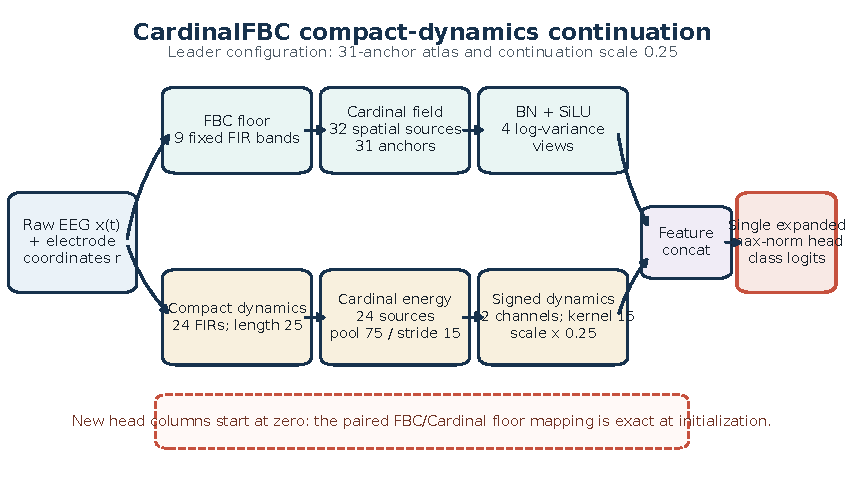
\includegraphics[width=0.98\textwidth]{figures/architecture.pdf}
\caption{Coordinate-field model and compact continuation. A nine-band FBC floor and a scaled energy/dynamics branch sample learned spatial weights at electrode coordinates. The continuation enters a single expanded max-norm head whose new columns start at zero, preserving the paired floor logits at initialization.}
\label{fig:architecture}
\end{figure*}

\subsection{Deployed Classical Decoders as Offline References}
\label{sec:classical}

The deployed decoders of Section~\ref{sec:online} were evaluated offline on the local cohort under their own deployment protocol (125~Hz, 8--30~Hz four-band causal filtering, 2.0-s epochs), which deliberately matches the online system rather than the harmonized benchmark profile. Two protocols were used. The personalized protocol is stratified five-fold cross-validation across each participant's four recordings, with per-recording alignment groups during fitting and the unsupervised set-reference step applied to each validation fold without labels---exactly the deployed calibration mechanism. The participant-independent protocol is leave-one-participant-out: the decoder is fitted on the seven other participants and aligned to the held-out participant only through the unsupervised reference step. The evaluation script and per-participant outputs accompany the manuscript sources.

In addition, the same classical decoders (plus a log-Euclidean tangent-anchor variant) are registered as a seedless, deterministic control protocol under the harmonized benchmark profile ($3\times448=1{,}344$ jobs); at manuscript freeze this grid was scheduled but unrun (0/1,344), so no classical score appears in the neural leaderboard. \textbf{[TODO: execute and audit the deterministic-control grid and add its protocol-separated table, or retain this status statement.]}

\subsection{Optimization, Refitting, and Determinism}

Every stochastic job used one of five fixed seeds: 7, 17, 27, 37, and 47. Models were trained for at most 200 epochs with batch size 64, AdamW learning rate $8\times10^{-4}$, weight decay $5\times10^{-4}$, cosine scheduling, patience 35, minimum improvement $10^{-4}$ in validation cross-entropy, label smoothing 0.05, and gradient-norm clipping at 5. Training augmentation used eight-segment reconstruction with probability 0.5, a temporal shift up to eight samples, and additive noise with standard deviation 0.01; reflection was disabled.

Before construction, each job reset all controlled random states. The source-training stage optimized training data only and chose the epoch count by validation cross-entropy. The implementation then reconstructed the exact seeded initial state and refitted on train plus validation for the selected number of epochs. The test partition was predicted once. Deterministic tensor operations were requested; these controls target computational repeatability within the frozen environment rather than bitwise identity across arbitrary hardware.

\subsection{Outcomes, Aggregation, and Exploratory Statistics}

Balanced accuracy was the primary outcome: the unweighted mean of class recalls. Raw accuracy, macro F1, Cohen's kappa, one-versus-rest macro area under the receiver-operating-characteristic curve, negative log likelihood, multiclass Brier score, and 15-bin expected calibration error were secondary outcomes. Trainable parameter count, inference milliseconds per trial, peak accelerator memory, and total job time were engineering outcomes.

The participant was the independent sampling unit. Prediction-only folds were concatenated within participant and seed; metrics were computed from the concatenated predictions, seeds were averaged within participant, participants were equally weighted within dataset, and the five dataset means were equally weighted. With $m_{ds}$ the seed-averaged metric for participant $s$ in dataset $d$, the reported estimand is
\begin{equation}
\widehat\mu=\frac{1}{5}\sum_{d=1}^{5}\frac{1}{n_d}\sum_{s=1}^{n_d}m_{ds}.
\label{eq:estimand}
\end{equation}

Participant-cluster bootstrap intervals used 100,000 deterministic resamples independently within each dataset while retaining equal dataset weights \cite{Efron1979}. One shared resample stream (seed 20260729) supplied the reported standard errors and figure intervals; the prespecified model-versus-TCFormer intervals reported in Section~\ref{sec:results} came from separate model-specific 100,000-resample streams. Because the reported leader was selected after observing 43 outcomes, its interval against TCFormer is descriptive rather than a confirmatory confidence interval.

We additionally performed an exploratory, post-hoc, one-sided paired sign-flip test for every one of the 42 non-TCFormer configurations against TCFormer. Within each resample, a shared random sign was applied to each participant's paired differences across the complete model family; participant means retained dataset stratification and equal dataset weights. The maximum unstudentized model-minus-TCFormer difference supplied a single-step resampling-based family-wise adjustment \cite{WestfallYoung1993}, with 100,000 Monte Carlo resamples, add-one $P$-value correction, and fixed seed 20260820. This test is a manuscript-level exploratory addition outside the frozen analysis contract, which itself reports no $P$ values; the adjustment addresses multiplicity within the observed 42-comparison family under sign symmetry but does not convert an opened, development-selected result into independent confirmation.

\section{Results}
\label{sec:results}

\subsection{Execution and Audit Completeness}

The common grid comprised 43 models, 448 participant/fold units, and five seeds, for 96,320 planned neural jobs. All 96,320 jobs completed; the immutable audit found zero failed, missing, or extra jobs. Each row retained cache and input identity, model identity, seed, selected epoch, timing, resources, metrics, and test probabilities required for deterministic aggregation. Complete 43-model balanced-accuracy and raw-accuracy tables, together with a 258-row (516-cell) reviewer replay catalog, accompany the release. The exact audit establishes table completeness under the registered common recipe, not external validity.

\subsection{Deployed Classical Decoders on the Local Cohort}

Table~\ref{tab:classical} reports the deployment-protocol evaluation of Section~\ref{sec:classical}. EA-FBCSP reached 91.1$\pm$6.3\% mean within-participant accuracy across the eight participants (range 78.8--97.9\%) and 86.4$\pm$8.2\% in the leave-one-participant-out protocol; the Riemannian tangent-space decoder reached 89.5$\pm$8.9\% and 82.8$\pm$10.1\%. Two observations follow. First, unsupervised reference realignment alone recovers most of the personalization gap for EA-FBCSP (4.8 points between protocols), supporting the platform's calibration-only deployment path for new users. Second, for context only, the best observed neural result on this cohort under the harmonized benchmark profile was 91.6\% balanced accuracy (Section~\ref{sec:heterogeneity}); because the deployment protocol differs in preprocessing, epoching, metric, and validation use, no rank or equivalence between classical and neural results is asserted here---the registered seedless control grid of Section~\ref{sec:classical} is the prespecified venue for that comparison.

\begin{table}[t]
\caption{Deployed Classical Decoders: Deployment-Protocol Accuracy on the Local Cohort (Mean $\pm$ SD Across Eight Participants)}
\label{tab:classical}
\centering
\scriptsize
\setlength{\tabcolsep}{4pt}
\begin{tabular}{lcc}
\toprule
Decoder & Personalized$^a$ & Participant-indep.$^b$ \\
\midrule
EA-FBCSP (2 comp.) + sLDA & 91.1 $\pm$ 6.3\% & 86.4 $\pm$ 8.2\% \\
Riemannian tangent + LR & 89.5 $\pm$ 8.9\% & 82.8 $\pm$ 10.1\% \\
\bottomrule
\multicolumn{3}{p{0.94\columnwidth}}{$^a$Stratified five-fold cross-validation over each participant's four recordings; label-free reference realignment per fold. $^b$Leave-one-participant-out with label-free reference realignment only. Deployment protocol (125 Hz, 8--30 Hz causal filter bank, 2.0-s epochs); not comparable cell-for-cell with the harmonized benchmark tables.} \\
\end{tabular}
\end{table}

\subsection{Effectiveness, Efficiency, and Calibration}

Table~\ref{tab:selected} reports the observed leader, the most accurate of the especially compact coordinate-field alternatives, TCFormer, and the paired FBCNet/CardinalFBC rows. The observed leader reached 73.990\% equal-dataset macro balanced accuracy and 74.021\% raw accuracy. TCFormer reached 73.316\% and 73.361\%, respectively. Their exploratory difference was 0.674 percentage points; the descriptive fixed-suite bootstrap interval ($-0.427$ to 1.899 points) crossed zero. The one-sided sign-flip test gave raw $P=0.152$ and all-42 maximum-difference adjusted $P=0.772$; the numerical ordering is therefore not evidence of confirmatory superiority.

The leader used a median 32,042 parameters, 57.65\% fewer than TCFormer's 75,668, and median inference was 14.38 times faster (ratios computed from unrounded medians). Median peak accelerator memory was 236.3 versus 606.6~MiB (61.05\% lower), and median total job time was 3.660 versus 42.964~s (11.74 times faster). The 13,523-parameter Sinc-based compact alternative reached 73.667\% balanced accuracy, a descriptive 0.351 points above TCFormer, with an interval that also crossed zero; it used 82.13\% fewer parameters and had 31.39 times lower median inference latency than TCFormer. At these budgets both models fit comfortably within the embedded latency envelope of the closed-loop platform of Section~\ref{sec:online}.

\begin{table*}[t]
\caption{Selected Common-Recipe Effectiveness and Efficiency Results}
\label{tab:selected}
\centering
\scriptsize
\setlength{\tabcolsep}{2.4pt}
\begin{tabular}{@{}p{3.15cm}r>{\raggedleft\arraybackslash}p{1.55cm}>{\raggedleft\arraybackslash}p{1.55cm}rp{2.45cm}p{2.30cm}r>{\raggedleft\arraybackslash}p{1.50cm}@{}}
\toprule
Model & Rank & \shortstack[r]{BA (\%)\\SE (pp)$^a$} & \shortstack[r]{Acc. (\%)\\SE (pp)$^a$} & $\Delta$TC (pp) & Exploratory 95\% interval (pp)$^b$ & Parameters, median [range] & Inference (ms/trial) & \shortstack[r]{ECE (\%)\\SE (pp)$^a$} \\
\midrule
Coordinate-field FBC + 0.25 compact dynamics, 31 anchors & 1 & \shortstack[r]{73.990\\(1.463)} & \shortstack[r]{74.021\\(1.463)} & 0.674 & [$-0.427$, 1.899] & 32,042 [31,850--35,116] & 0.1210 & \shortstack[r]{14.285\\(0.547)} \\
Sinc coordinate dynamics, 31 anchors & 3 & \shortstack[r]{73.667\\(1.494)} & \shortstack[r]{73.674\\(1.494)} & 0.351 & [$-0.778$, 1.518] & 13,523 [13,331--14,389] & 0.0554 & \shortstack[r]{9.085\\(0.297)} \\
TCFormer & 12 & \shortstack[r]{73.316\\(1.742)} & \shortstack[r]{73.361\\(1.741)} & 0 & Reference & 75,668 [72,212--75,804] & 1.7390 & \shortstack[r]{6.976\\(0.469)} \\
FBCNet & 19 & \shortstack[r]{73.205\\(1.423)} & \shortstack[r]{73.240\\(1.423)} & $-0.111$ & [$-1.218$, 1.086] & 9,218 [4,034--11,524] & 0.0798 & \shortstack[r]{14.289\\(0.485)} \\
Coordinate-field FBC floor & 20 & \shortstack[r]{73.201\\(1.473)} & \shortstack[r]{73.236\\(1.473)} & $-0.115$ & [$-1.201$, 1.026] & 9,218 [9,218--11,524] & 0.0874 & \shortstack[r]{14.189\\(0.452)} \\
\bottomrule
\multicolumn{9}{p{17.3cm}}{$^a$Estimate with bootstrap standard error beneath: sample standard deviation of 100,000 participant-stratified replicate equal-dataset estimates. $^b$Model minus prespecified TCFormer; model-specific 100,000-resample participant-cluster bootstrap on the opened development suite. Intervals are descriptive, unadjusted for selection or multiplicity, and are not confirmatory confidence intervals. Omitted ranks 2 and 4--10 are additional in-house coordinate-field configurations and rank 11 is FBMSNet; the released tables report all 43 models. BA, balanced accuracy; Acc., raw accuracy; ECE, 15-bin expected calibration error.} \\
\end{tabular}
\end{table*}

FBCNet and its coordinate-field floor both used a median 9,218 parameters and differed by only 0.004 balanced-accuracy points overall (73.201 versus 73.205). Thus, the present grid does not isolate a benefit from replacing the indexed FBC spatial convolution alone; the leader's improvement could reflect the continuation, the 31-anchor support, their optimization interaction, or outcome selection among configurations. Figure~\ref{fig:efficiency} places all 43 models in the balanced-accuracy/parameter plane. Descriptively, the ten highest balanced accuracies belonged to in-house coordinate-field configurations, with the highest-ranked public models (FBMSNet, TCFormer) at ranks 11--12; ranks 10--12 were separated by less than 0.002 points, so this family-level ordering is an observation about this grid rather than a meaningful separation.

The calibration ranking differed from the balanced-accuracy ranking. TCFormer had the lowest selected-row expected calibration error (6.976\%; SE 0.469 points), negative log likelihood (0.503; SE 0.031), and Brier score (0.321; SE 0.019). The leader's corresponding values were 14.285\% (SE 0.547 points), 0.626 (SE 0.028), and 0.369 (SE 0.018). The compact Sinc alternative was intermediate at 9.085\% (SE 0.297 points), 0.515 (SE 0.026), and 0.330 (SE 0.017). Efficiency and discrimination therefore did not remove the need to assess probability quality.

\begin{figure}[t]
\centering
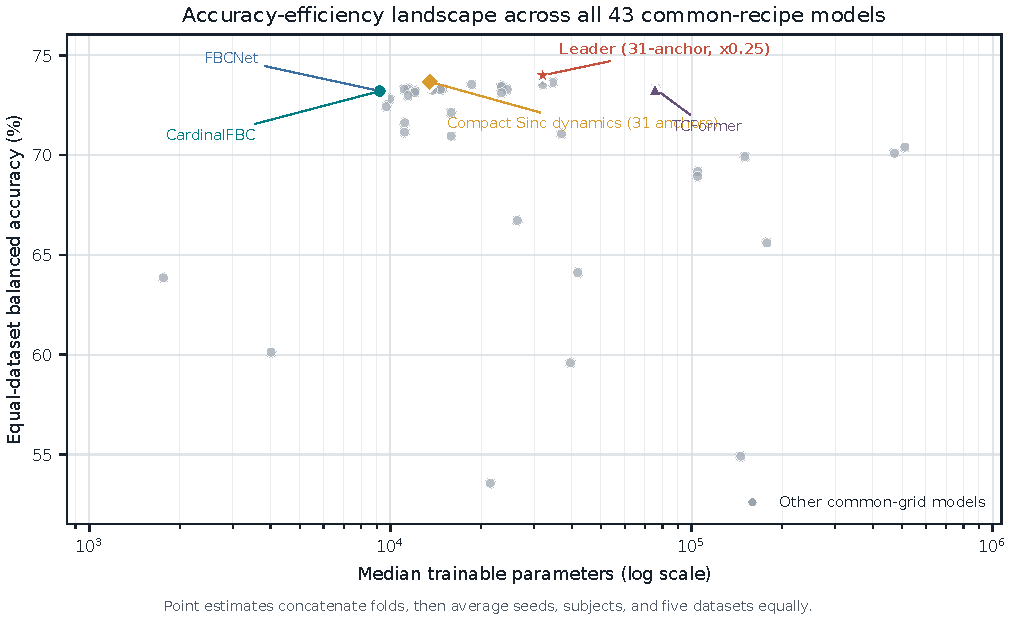
\includegraphics[width=\columnwidth]{figures/efficiency_scatter.pdf}
\caption{All-model performance--efficiency context. Equal-dataset macro balanced accuracy is plotted against median trainable parameter count for all 43 common-recipe configurations; selected models are labeled. Parameter counts vary with input channels and class count, so medians and ranges accompany tabulated values.}
\label{fig:efficiency}
\end{figure}

\subsection{Dataset Heterogeneity}
\label{sec:heterogeneity}

Figure~\ref{fig:deltas} reports dataset-specific paired differences with participant-cluster bootstrap intervals; the overall average combines effects with different signs and magnitudes. Relative to TCFormer, the leader's difference was positive on BNCI2014-001 and Cho2017, near zero on Local Exp4 and BNCI2014-004, and negative on PhysioNet. The compact alternative was numerically higher than TCFormer on Local Exp4, BNCI2014-004, and PhysioNet but lower on BNCI2014-001 and Cho2017. On the local platform cohort, the best observed benchmark result under the common recipe was the compact Sinc model at 91.6\% balanced accuracy. No selected model was the best observed model on every dataset; absolute dataset estimates and their resampling uncertainty are retained in the machine-readable statistics record.

\begin{figure}[t]
\centering
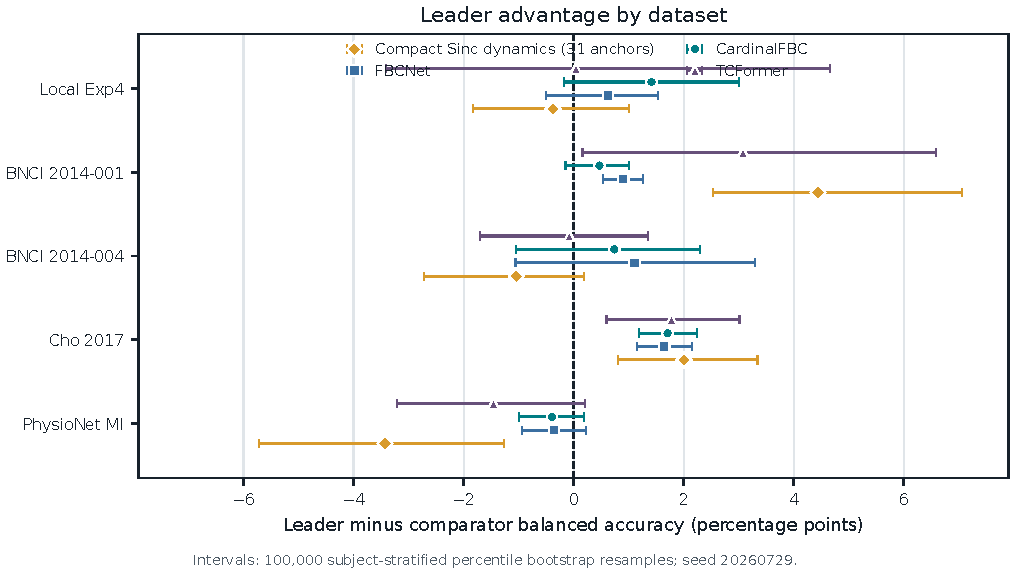
\includegraphics[width=\columnwidth]{figures/dataset_deltas.pdf}
\caption{Dataset-specific balanced-accuracy differences between the observed leader and each selected comparator. Positive values favor the leader. Points are participant-equal mean differences and bars are descriptive participant-cluster bootstrap intervals for the fixed opened suite; they are not selection-adjusted confirmatory intervals.}
\label{fig:deltas}
\end{figure}

\section{Discussion}
\label{sec:discussion}

The platform results and the benchmark results answer complementary questions. The deployment evaluation shows that a complete, low-cost MI-BCI chain---consumer amplifier, scripted cue acquisition, aligned classical decoding, unsupervised in-context calibration, and conservative evidence gating---supports accurate discrete control: 91\% within-participant accuracy, 86\% for new users with calibration only, and completed closed-loop navigation in pilot sessions. The benchmark asks what neural architectures add on top of such a chain, and under what resource budget.

The principal benchmark observation is an accuracy--resource tradeoff, not a superiority result. Under one frozen recipe, a coordinate-field FBC continuation produced the largest observed equal-dataset balanced accuracy while using 42\% of the median parameters, 7\% of the inference time, and 39\% of the accelerator memory of TCFormer, and the 13,523-parameter coordinate-dynamics model was close behind at 18\% of TCFormer's parameters. These resource differences are meaningful engineering measurements within the audited environment, but latency and memory depend on hardware and software versions and should be remeasured on any deployment target.

The architectural evidence is narrower than the leaderboard. The coordinate field turns learned anchor coefficients into spatial weights at recorded coordinates, and the zero-start continuation initially preserves the paired FBC logits---a coherent implementation of coordinate-conditioned weights and a controlled way to add dynamics features. However, CardinalFBC alone was essentially tied with FBCNet, so the experiments do not show that coordinate parameterization by itself caused the leader's score; the 31-anchor atlas is an architectural support ablation rather than proof of cross-montage generalization. No experiment here changed the voltage reference, evaluated arbitrary missing channels, or trained on one montage and confirmed on an untouched different one.

Dataset effects were heterogeneous. The leader's largest positive difference from TCFormer occurred on the four-class BNCI2014-001 task, whereas TCFormer was numerically higher on PhysioNet, where both methods sat much closer to chance than on the other binary cohorts. Equal dataset weighting prevents the two large cohorts from dominating the three smaller ones, but it defines a fixed-suite estimand rather than the prevalence-weighted performance of a clinical population. Calibration revealed a further tradeoff: TCFormer produced better probability quality than the accuracy leader, which matters for downstream systems---including ours---that threshold confidence before acting. No post-hoc calibration method was fitted because the frozen recipe did not include one; future work should predefine calibration and evaluate it without test reuse.

Several limitations bound the claims. All five cohorts were opened during development; none is independent confirmation, and PhysioNet S55--S109 and other registered cohorts remain sealed until a confirmation protocol is frozen. Selecting the best of 43 configurations makes an unadjusted contrast optimistic; the exploratory all-42 maximum-difference test accounts for the comparison family under sign symmetry but was designed after the outcomes were available, and its adjusted $P$ value (0.772) was consistent with no detectable family-wise advantage. The harmonized classical-control grid is pending, so classical and neural rows do not yet share one protocol; the deployment-protocol classical results, while computed with leakage-controlled cross-validation, use the platform's own preprocessing and are not leaderboard rows. Finally, the common training recipe improves comparability but may disadvantage public models whose author recipes differ; an author-recipe comparison is registered as separate future work. The most useful next experiment is a prespecified confirmation of a frozen small set---the leader, the compact alternative, TCFormer, FBCNet, and the completed classical controls---with a defined participant-level effect, multiplicity control, and calibration outcome, on data untouched during development.

\section{Conclusion}
\label{sec:conclusion}

This work documented a complete motor-imagery BCI platform and evaluated its decoders under auditable protocols. The deployed classical pipeline---Euclidean-aligned FBCSP or Riemannian tangent-space decoding with unsupervised in-context calibration and temporal evidence gating---reached 91.1$\pm$6.3\% within-participant and 86.4$\pm$8.2\% participant-independent accuracy on the locally acquired cohort and completed closed-loop navigation in pilot sessions. The accompanying 96,320-job benchmark of 43 neural configurations across five cohorts identified a coordinate-field FBC model with a zero-start compact-dynamics continuation as the highest-scoring observed configuration at 73.99\% equal-dataset balanced accuracy, with a 13,523-parameter coordinate-dynamics alternative at 73.67\%; the 75,668-parameter TCFormer reference reached 73.32\% with better calibration. The in-house leaders used less than half of the reference's parameters and an order of magnitude less inference time, but their exploratory intervals against TCFormer included zero and dataset effects were heterogeneous, so the results support efficiency-competitive candidates and a reproducible evaluation procedure rather than confirmed superiority. Before submission-grade claims can be extended, the study requires the completed classical-control grid, independent verification of the exploratory statistics, a prespecified test on untouched confirmation data, and resolution of the local cohort's ethics and data-governance record. The platform description, frozen seeds, per-job audit, and protocol-separated outputs provide the foundation for that confirmation.

\section*{Ethics and Human-Participant Protection}

Local Exp4 recordings were acquired with a non-invasive, consumer-grade surface-EEG amplifier under the cue protocol of Section~\ref{sec:platform}, and participants are identified in all artifacts only by pseudonymous codes. \textbf{[TODO---RELEASE BLOCKER: insert the verified ethics statement: institution, protocol identifier, approval/exemption status, consent basis, and compliance with applicable human-participant standards; state the ethics and consent provenance reported by each public dataset source.]}

\section*{Data and Code Availability}

Public datasets must be reacquired from their authoritative records under their exact terms; raw EEG and transformed caches are not distributed with the project. Local Exp4 recordings are private pending institutional authorization. The release accompanying this manuscript contains aggregate metrics, per-job audit identities, cryptographic hashes, the deterministic analysis and asset-generation scripts, and the deployment-protocol classical evaluation script and outputs. \textbf{[TODO: insert the final repository identifier, immutable release tag, environment lock hash, and project software license.]}

\section*{Acknowledgment, Funding, and Conflicts}

All reported numbers derive from the audited artifacts described above. \textbf{[TODO: identify every funding source and grant; disclose or explicitly deny conflicts of interest; disclose the companion closed-loop manuscript and any preliminary abstracts.]}

\IEEEtriggeratref{25}
\bibliographystyle{IEEEtran}
\bibliography{references}

\end{document}
